\documentclass[12pt, a4paper, simple]{eskdtext}

\usepackage{config/main.env}
\usepackage{config/report.env}
\usepackage{styles/listing}
\usepackage{styles/lists}
\usepackage{styles/SectionMargins}
\usepackage{styles/table}
\usepackage{styles/TableOfContent}
\usepackage{styles/url}

\begin{document}
  \begin{ESKDtitlePage}
  \ESKDstyle{empty}
  \begin{center}
    \envReportMinistr \\
    \envReportEducation \\
    \envReportUniversity \\
    \envReportCathedra \\
  \end{center}

  \vfill

  \begin{center}
    Тема: <<\envReportTitle>>
  \end{center}

  \vfill

  \begin{center}
    Отчёт лабораторной работы №\envReportLabNumber \\
    по дисциплине \envReportSubject \\
  \end{center}

  \vfill

  \begin{flushright}
    \begin{minipage}[t]{7cm}
      Выполнил: \\
      \envReportStudentInfo \\
      \hspace{0pt} \\
      Проверил: \\
      \envReportTeacherInfo \\
    \end{minipage}
  \end{flushright}

  \vfill

  \begin{center}
    \envReportCity~\ESKDtheYear
  \end{center}
\end{ESKDtitlePage}


  % = = = = = = = = = = = = = = = =
  \ESKDstyle{empty}
  \begin{center}
    \textbf{Отчёт лабораторной работы №\envReportLabNumber}
  \end{center}

  \paragraph{} \textbf{Тема}: <<\envReportTitle>>

  \paragraph{} \textbf{Цель}:
  Знакомство с Kubernetes Engine, Container Registry.

  \paragraph{} \textbf{Что нужно сделать}:

  Полученные в предыдущей работе образы должны быть запущены в Google Kubernetes Engine.
  Для этого сохраните их в Google Container Registry.

  Для создания и управления кластером используйте kubectl.
  Настройте все взаимодействия между сервисами.

  После запуска убедитесь в BigQuery, Cloud Functions, что общая система продолжает функционировать,
  несмотря на переезд микросервисов из GCE и GAE в GKE.

  \paragraph{} \textbf{{Ход работы}}:

  Посмотрел видео на YouTube \cite{kubernetes_install} по установке VirtualBox, kubectl, minikube на Win10.

  \begin{lstlisting}[
    frame=single,
    rulecolor=\color{blue},
    name={Установка VirtualBox на Ubuntu 22.10},
  ]
sudo apt update
sudo apt install virtualbox
\end{lstlisting}

  Почитал официальную документацию \cite{kubernetes_install_kubectl} и установил kubectl.

\begin{lstlisting}[
  frame=single,
  rulecolor=\color{blue},
  name={Установка kubectl на Ubuntu 22.10},
]
curl -LO "https://dl.k8s.io/release/$(curl -L -s https://dl.k8s.io/release/stable.txt)/bin/linux/amd64/kubectl"
curl -LO "https://dl.k8s.io/$(curl -L -s https://dl.k8s.io/release/stable.txt)/bin/linux/amd64/kubectl.sha256"
echo "$(cat kubectl.sha256)  kubectl" | sha256sum --check
sudo install -o root -g root -m 0755 kubectl /usr/local/bin/kubectl
kubectl version --client
\end{lstlisting}

  Почитал официальную документацию \cite{kubernetes_install_minikube} и установил minikube.

\begin{lstlisting}[
  frame=single,
  rulecolor=\color{blue},
  name={Установка minikube на Ubuntu 22.10},
]
curl -LO https://storage.googleapis.com/minikube/releases/latest/minikube-linux-amd64
sudo install minikube-linux-amd64 /usr/local/bin/minikube
minikube version
\end{lstlisting}

  Посмотрел теорию на YouTube \cite{kubernetes_theory} по Kubernetes.

  Посмотрел практику по подам Kubernetes на YouTube \cite{kubernetes_create_pod} и создал конфиги pod-ms3-ver1.yaml, pod-ms2-ver1.yaml.

  \newpage
  \lstinputlisting[
    frame=single,
    rulecolor=\color{magenta},
  ]{../sources/K8S/pod-ms3-ver1.example.yaml}

  \begin{lstlisting}[
    frame=single,
    rulecolor=\color{blue},
    name={Запуск пода MS3},
  ]
cp pod-ms3-ver1.example.yaml pod-ms3-ver1.yaml

# меняем настройки env в файле pod-ms3-ver1.yaml

kubectl apply -f pod-ms3-ver1.yaml  # запускаем под

kubectl get pods                    # смотрим активные поды
kubectl describe pods ms3           # больше информации о MS3
kubectl logs ms3                    # смотрим логи MS3
kubectl port-forward ms3 3333:8080  # открываем порт на своей машине

kubectl get pods                    # смотрим активные поды
kubectl delete -f pod-ms3-ver1.yaml # удаляем под kubectl delete pods ms3
kubectl get pods                    # смотрим активные поды
\end{lstlisting}

  \newpage

  \lstinputlisting[
    frame=single,
    rulecolor=\color{magenta},
  ]{../sources/K8S/pod-ms2-ver1.example.yaml}

  \newpage

  \begin{lstlisting}[
    frame=single,
    rulecolor=\color{blue},
    name={Запуск пода MS2},
  ]
cp pod-ms2-ver1.example.yaml pod-ms2-ver1.yaml

# меняем настройки env в файле pod-ms2-ver1.yaml

kubectl apply -f pod-ms2-ver1.yaml  # запускаем под

kubectl get pods                    # смотрим активные поды
kubectl describe pods ms2           # больше информации о MS2
kubectl logs ms2                    # смотрим логи MS2
kubectl port-forward ms2 2222:44480 # открываем порт на своей машине

kubectl get pods                    # смотрим активные поды
kubectl delete -f pod-ms2-ver1.yaml # удаляем под kubectl delete pods ms2
kubectl get pods                    # смотрим активные поды
\end{lstlisting}

\begin{center}
  \textbf{Создание кластера в Google Cloud Kubernetes Engine}
\end{center}

\begin{lstlisting}[
  language=bash,
  frame=single,
  rulecolor=\color{blue},
  name={Создание кластера в Google Cloud Kubernetes Engine},
]
gcloud init                                                 # соединяемся с Google Cloud
gcloud services enable container.googleapis.com             # включаем Google API

gcloud container clusters create rsiot-po4-190333-cluster   # создаем кластер

gcloud components install gke-gcloud-auth-plugin            # установка SDK для работы с kubectl

gcloud container clusters get-credentials rsiot-po4-190333-cluster  # переключаемся на кластер  
\end{lstlisting}

\begin{lstlisting}[
  frame=single,
  rulecolor=\color{blue},
  name={Терминал},
]
kubectl cluster-info
\end{lstlisting}

\begin{lstlisting}[
  frame=single,
  rulecolor=\color{green},
  name={Вывод в терминал},
]
Kubernetes control plane is running at https://35.184.161.203
GLBCDefaultBackend is running at https://35.184.161.203/api/v1/namespaces/kube-system/services/default-http-backend:http/proxy
KubeDNS is running at https://35.184.161.203/api/v1/namespaces/kube-system/services/kube-dns:dns/proxy
Metrics-server is running at https://35.184.161.203/api/v1/namespaces/kube-system/services/https:metrics-server:/proxy

To further debug and diagnose cluster problems, use 'kubectl cluster-info dump'.   
\end{lstlisting}

\begin{lstlisting}[
  frame=single,
  rulecolor=\color{blue},
  name={Терминал},
]
kubectl get componentstatuses 
\end{lstlisting}

\begin{lstlisting}[
  frame=single,
  rulecolor=\color{green},
  name={Вывод в терминал},
]
NAME                 STATUS    MESSAGE             ERROR
controller-manager   Healthy   ok                  
scheduler            Healthy   ok                  
etcd-0               Healthy   {"health":"true"}   
etcd-1               Healthy   {"health":"true"}  
\end{lstlisting}

\newpage

\begin{lstlisting}[
  frame=single,
  rulecolor=\color{blue},
  name={Терминал},
]
kubectl get nodes
\end{lstlisting}

\begin{lstlisting}[
  frame=single,
  rulecolor=\color{green},
  name={Вывод в терминал},
]
NAME                                                  STATUS   ROLES    AGE    VERSION
gke-rsiot-po4-190333-clu-default-pool-e4446c63-hmnz   Ready    <none>   6m8s   v1.24.9-gke.3200
gke-rsiot-po4-190333-clu-default-pool-e4446c63-js81   Ready    <none>   6m9s   v1.24.9-gke.3200
gke-rsiot-po4-190333-clu-default-pool-e4446c63-xrnh   Ready    <none>   6m9s   v1.24.9-gke.3200
\end{lstlisting}

  Заходим на сайт Google Cloud Console \cite{GoogleCloudConsole} (см. рисунок~\ref{fig:1}).

  Menu > Compute Engine > VM instances (см. рисунок~\ref{fig:1}).

  Видем, что у нас создалось три компьютера в кластере (см. рисунок~\ref{fig:2}).

  \begin{figure}[!h]
    \centering

    \begin{minipage}{0.49\textwidth}
      \centering

      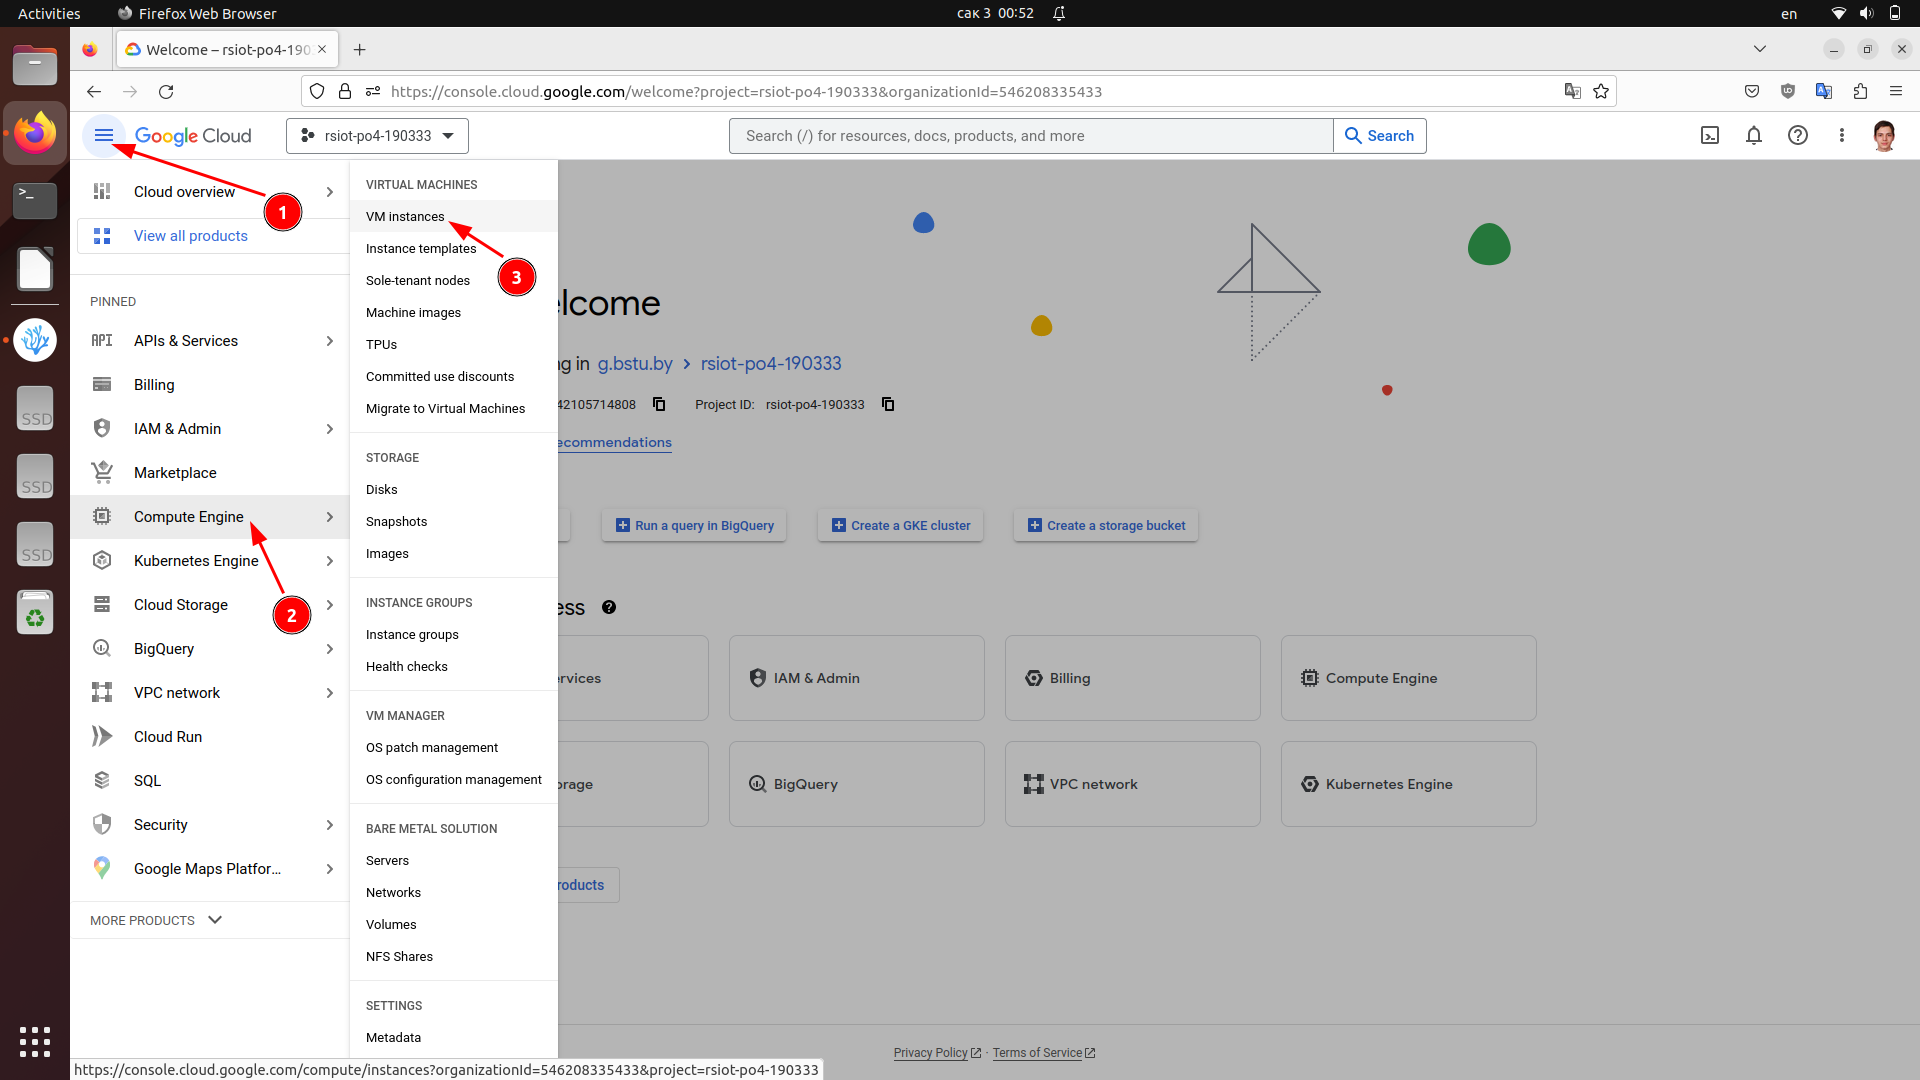
\includegraphics[height=5cm]
      {images/2023-03-03_00-53-23.png}

      \caption{\_}

      \label{fig:1}
    \end{minipage}
    \begin{minipage}{0.49\textwidth}
      \centering

      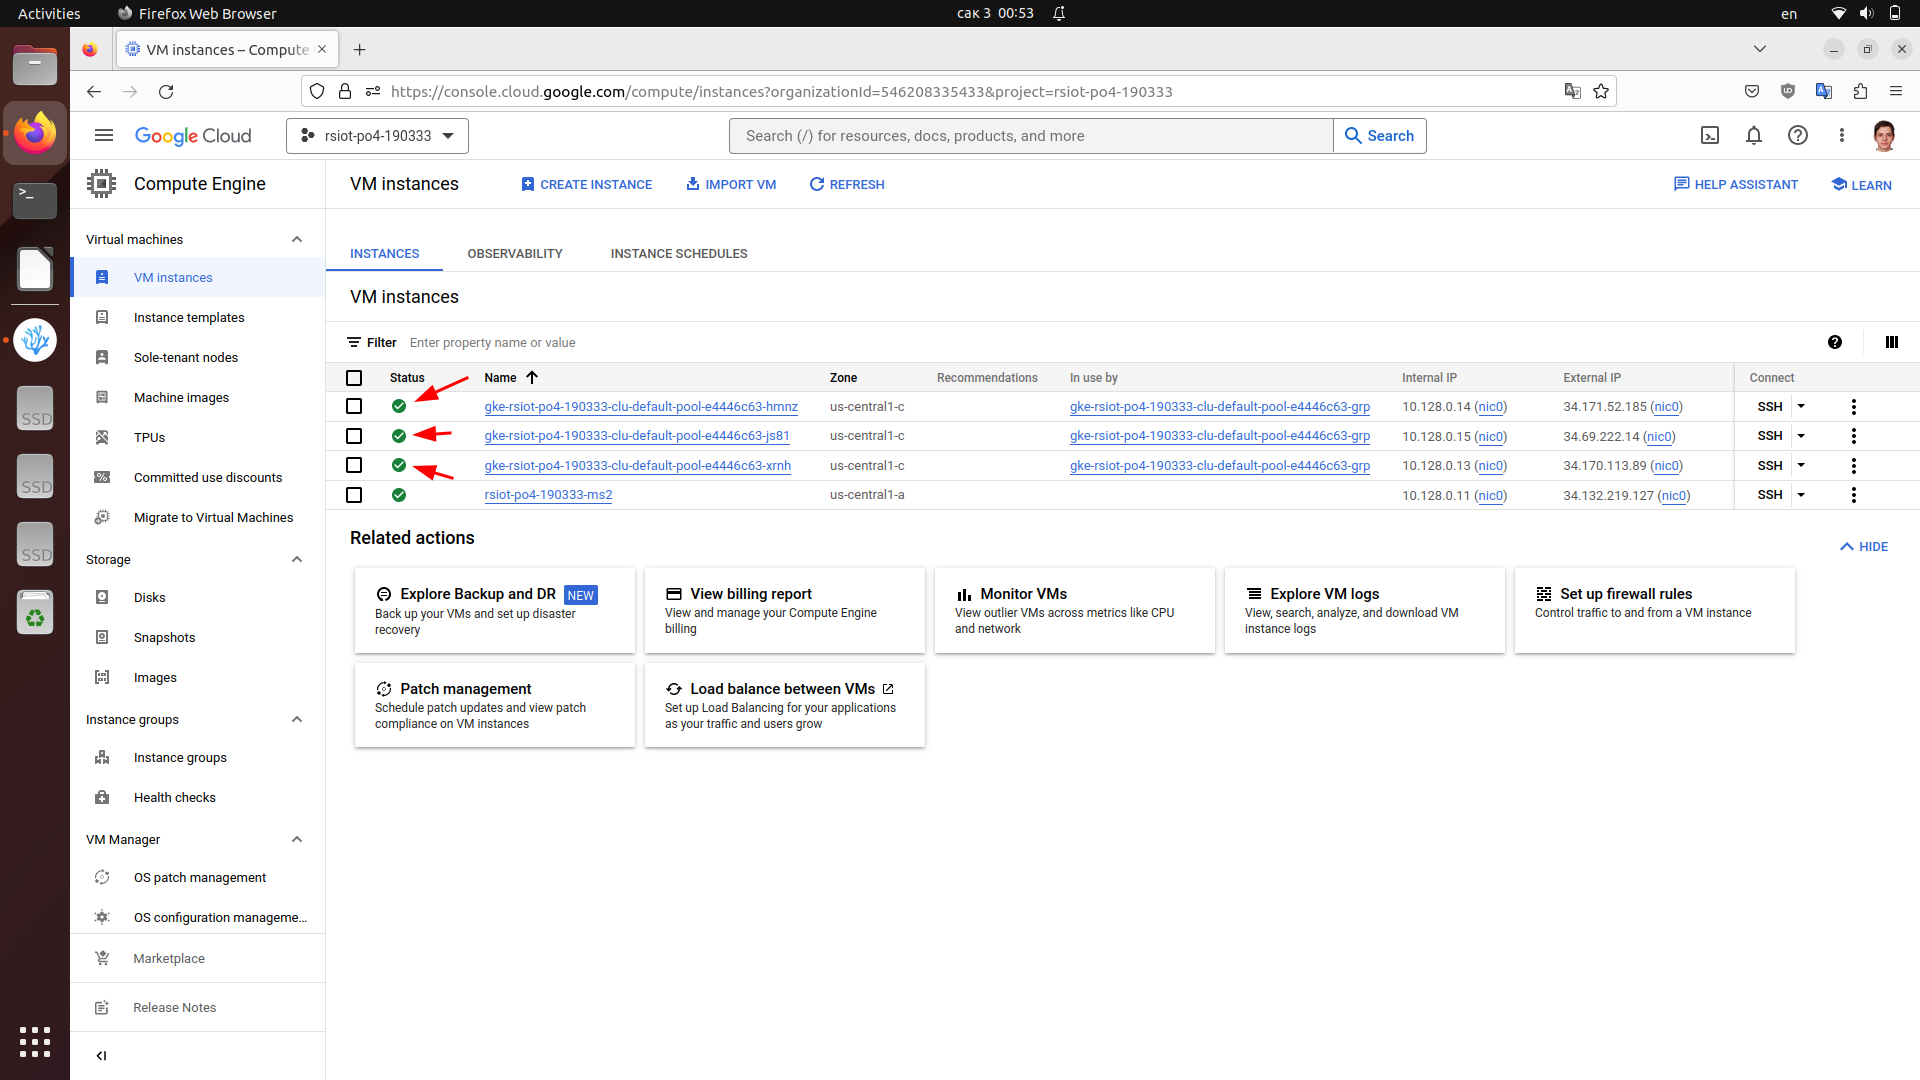
\includegraphics[height=5cm]
      {images/2023-03-03_00-53-56.png}

      \caption{\_}

      \label{fig:2}
    \end{minipage}
  \end{figure}

  Заходим на сайт Google Cloud Console \cite{GoogleCloudConsole} (см. рисунок~\ref{fig:3}).

  Menu > Kubernetes Engine > Clasters (см. рисунок~\ref{fig:3}).

  Видем, что у нас создался кластер (см. рисунок~\ref{fig:4}).

  \begin{figure}[!h]
    \centering

    \begin{minipage}{0.49\textwidth}
      \centering

      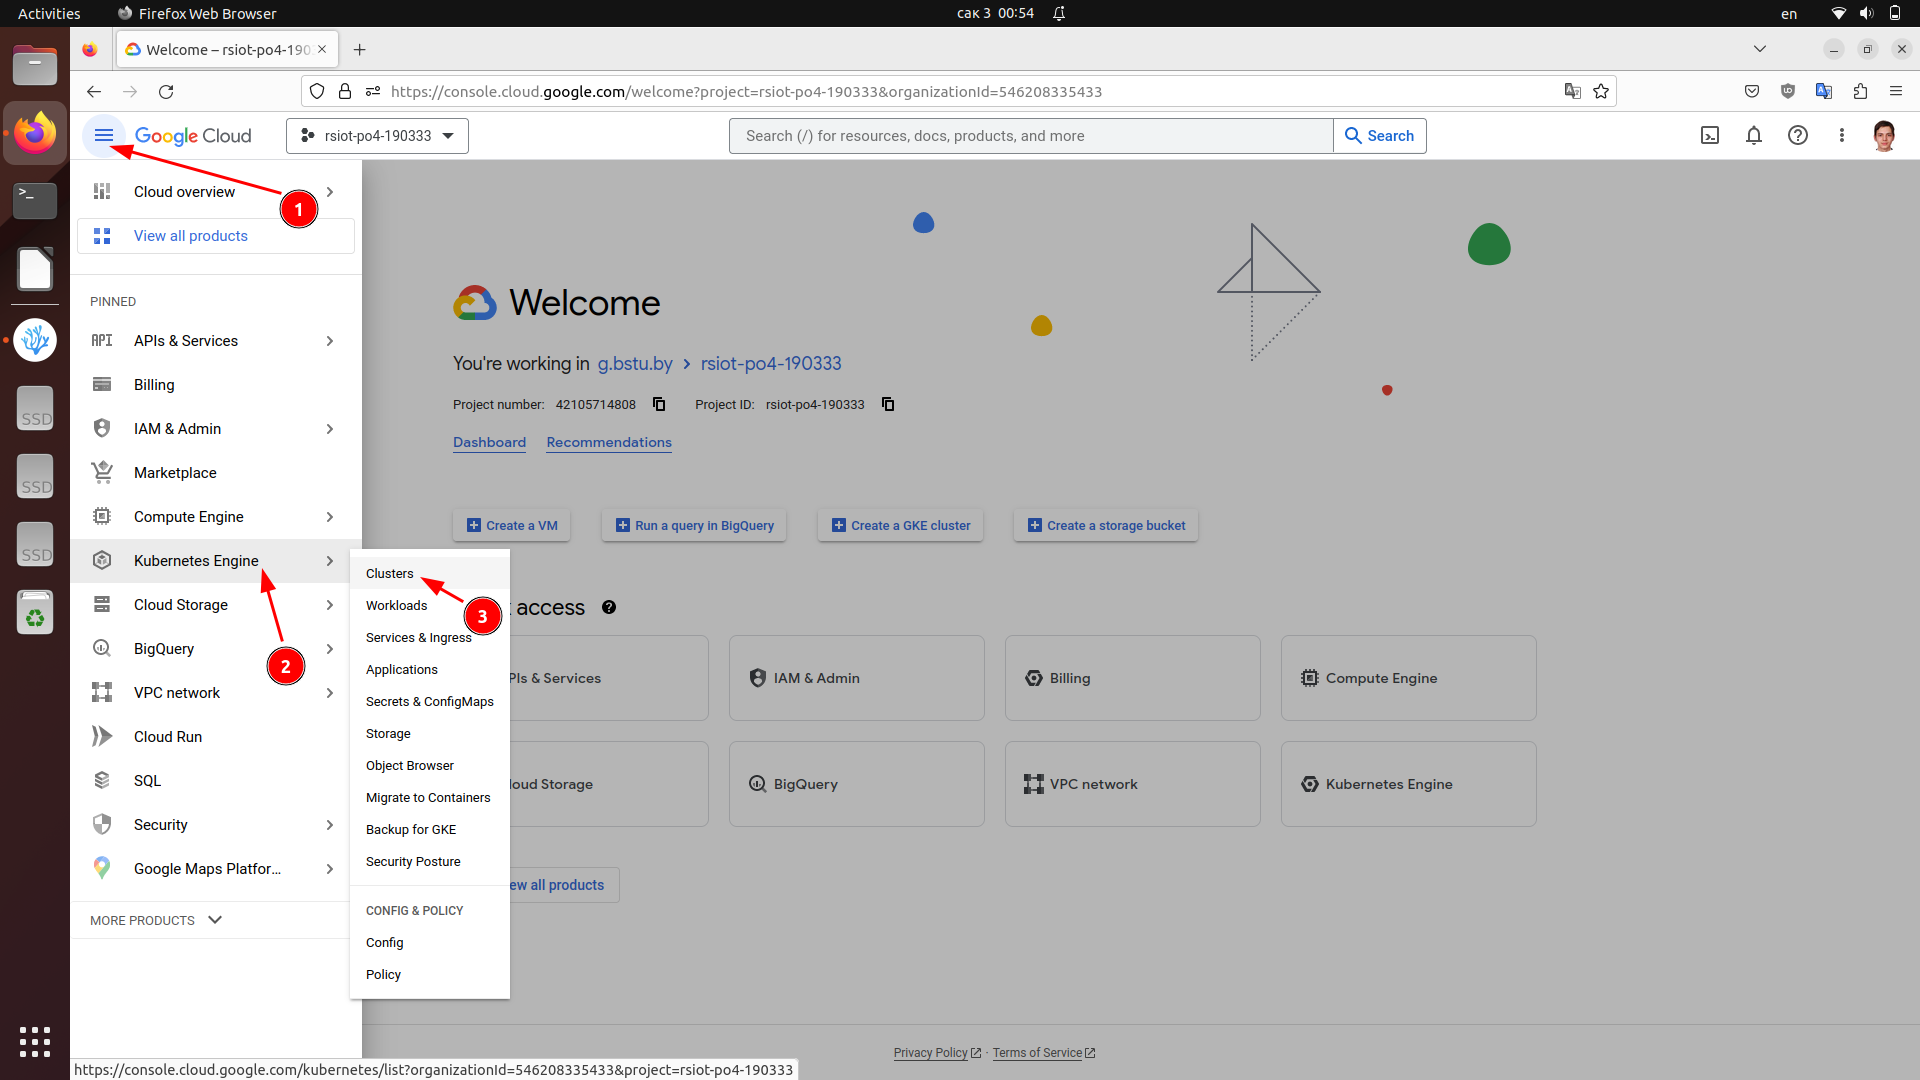
\includegraphics[height=5cm]
      {images/2023-03-03_00-54-36.png}

      \caption{\_}

      \label{fig:3}
    \end{minipage}
    \begin{minipage}{0.49\textwidth}
      \centering

      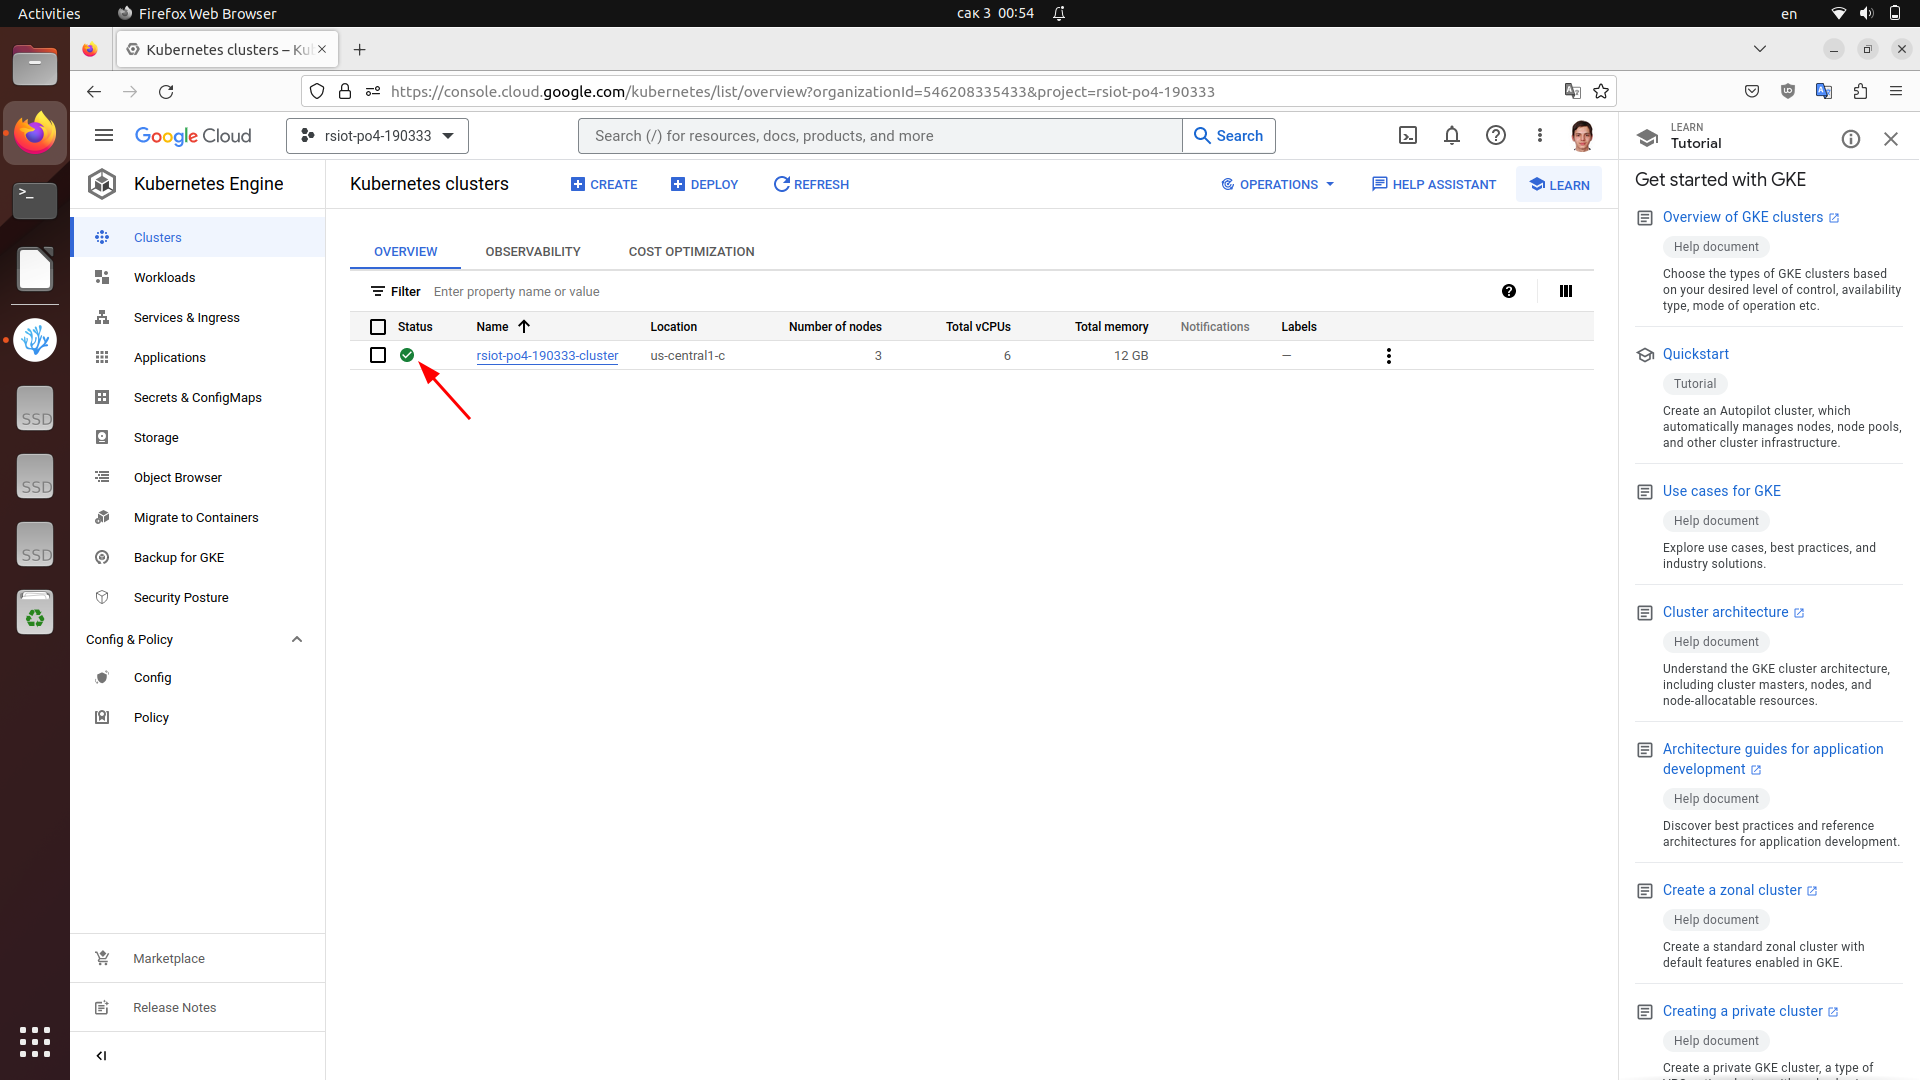
\includegraphics[height=5cm]
      {images/2023-03-03_00-54-54.png}

      \caption{\_}

      \label{fig:4}
    \end{minipage}
  \end{figure}

  \newpage

  \begin{center}
    \textbf{Создание deployment в Google Cloud Kubernetes Engine для MS3}
  \end{center}

  \begin{lstlisting}[
    language=bash,
    frame=single,
    rulecolor=\color{blue},
    name={Терминал},
  ]
gcloud container clusters get-credentials rsiot-po4-190333-cluster

kubectl apply -f deployment-ms3.yaml # создаем deployment из конфига
kubectl get pods        # ждем когда будет статус Running, а не ContainerCreating
kubectl get deployments # смотрим, что создался deployment

# Можно открыть в браузере http://35.224.214.112:8080:
kubectl expose deployment ms3-deployment --type=LoadBalancer --port=8080 --target-port=8080

# Можно открыть в браузере http://localhost:8888:
# $ kubectl port-forward ms3-deployment-7bbb9d8ff9-fdqzh 8888:8080

# Удалить deployment: $ kubectl delete -f deployment-ms3.yaml
\end{lstlisting}

  \lstinputlisting[
    frame=single,
    rulecolor=\color{magenta},
  ]{../sources/K8S/deployment-ms3.example.yaml}

  Как создать deployment смотрел по видео на YouTube \cite{kubernetes_create_deployment}.

  Заходим на сайт Google Cloud Kubernetes Engine \cite{GoogleCloudConsole} (см. рисунок~\ref{fig:5}).

  Жмём <<Workloads>> - и видем, что у нас запущен ms3-deployment (см. рисунок~\ref{fig:5}).

  Жмём <<Services \& Ingress>> - и видем, что у нас открыт порт (см. рисунок~\ref{fig:6}).

  \begin{figure}[!h]
    \centering

    \begin{minipage}{0.49\textwidth}
      \centering

      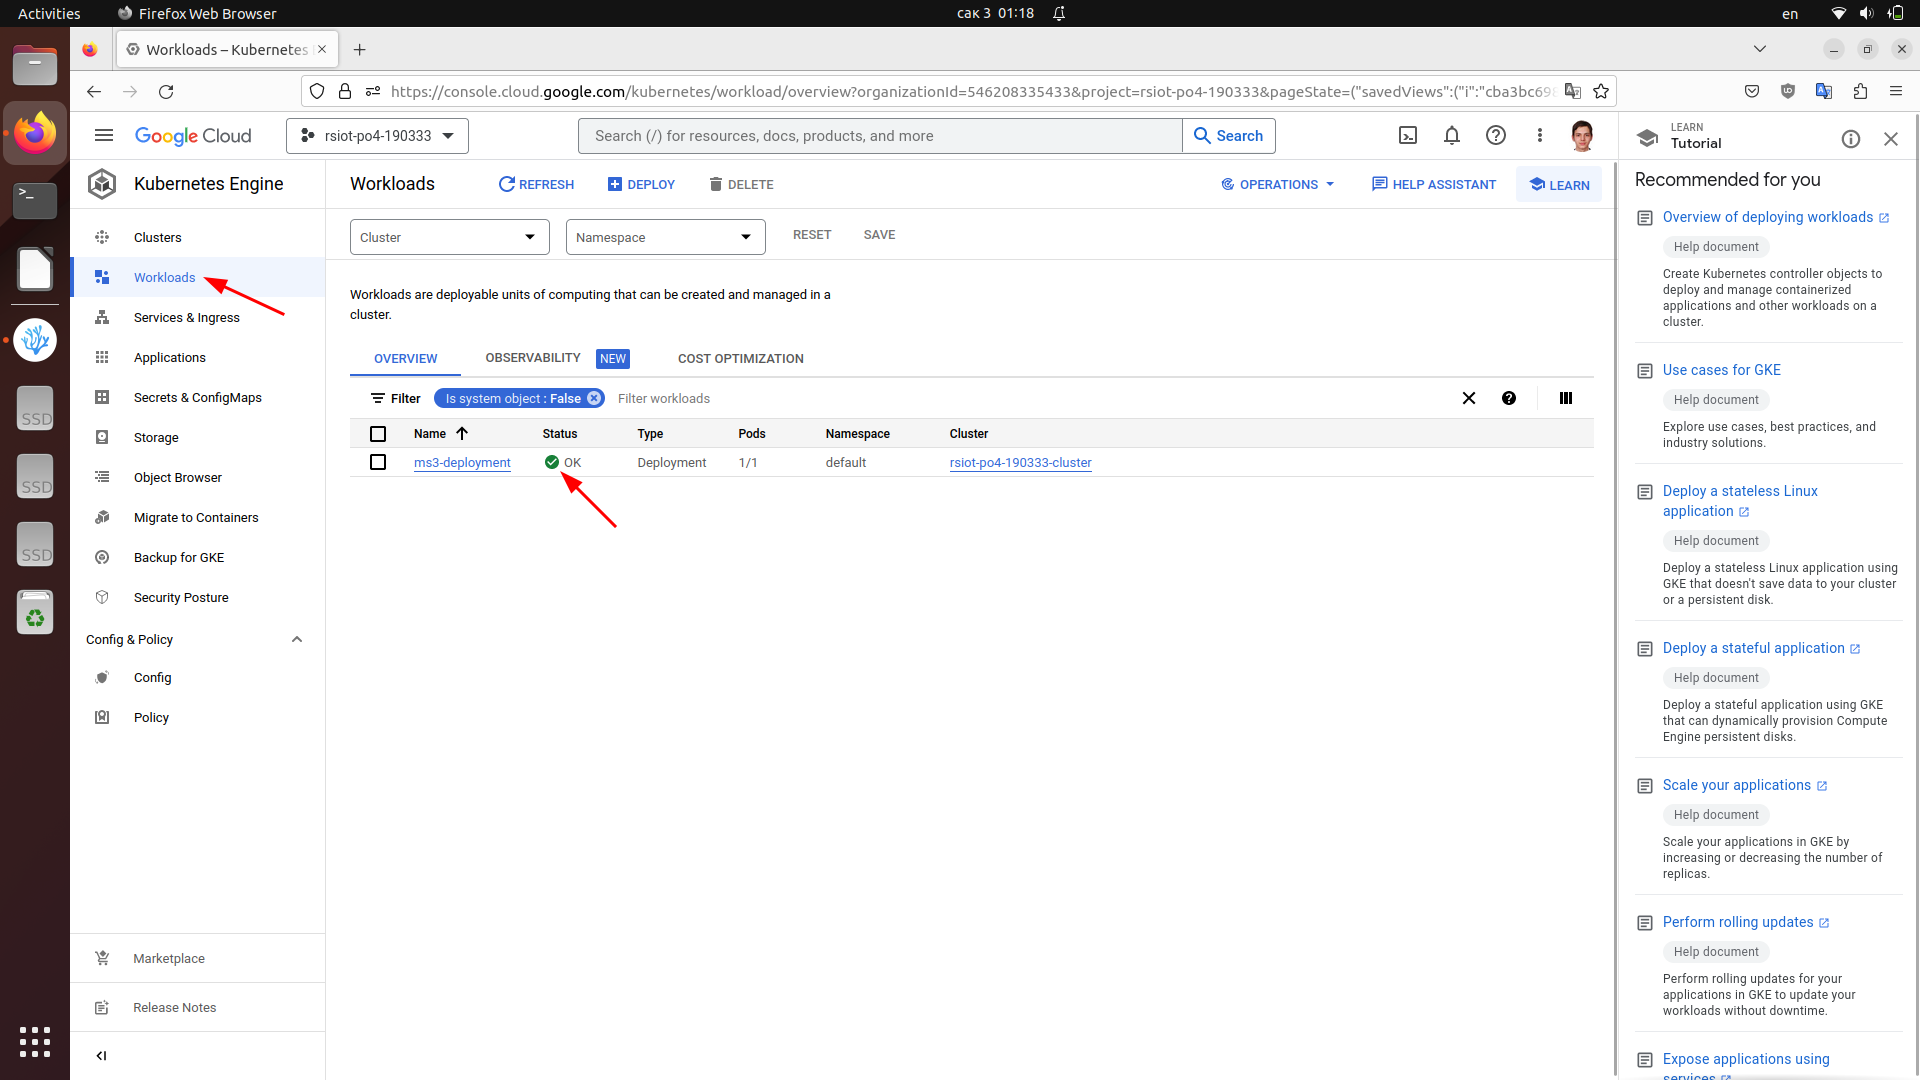
\includegraphics[height=5cm]
      {images/2023-03-03_01-18-40.png}

      \caption{\_}

      \label{fig:5}
    \end{minipage}
    \begin{minipage}{0.49\textwidth}
      \centering

      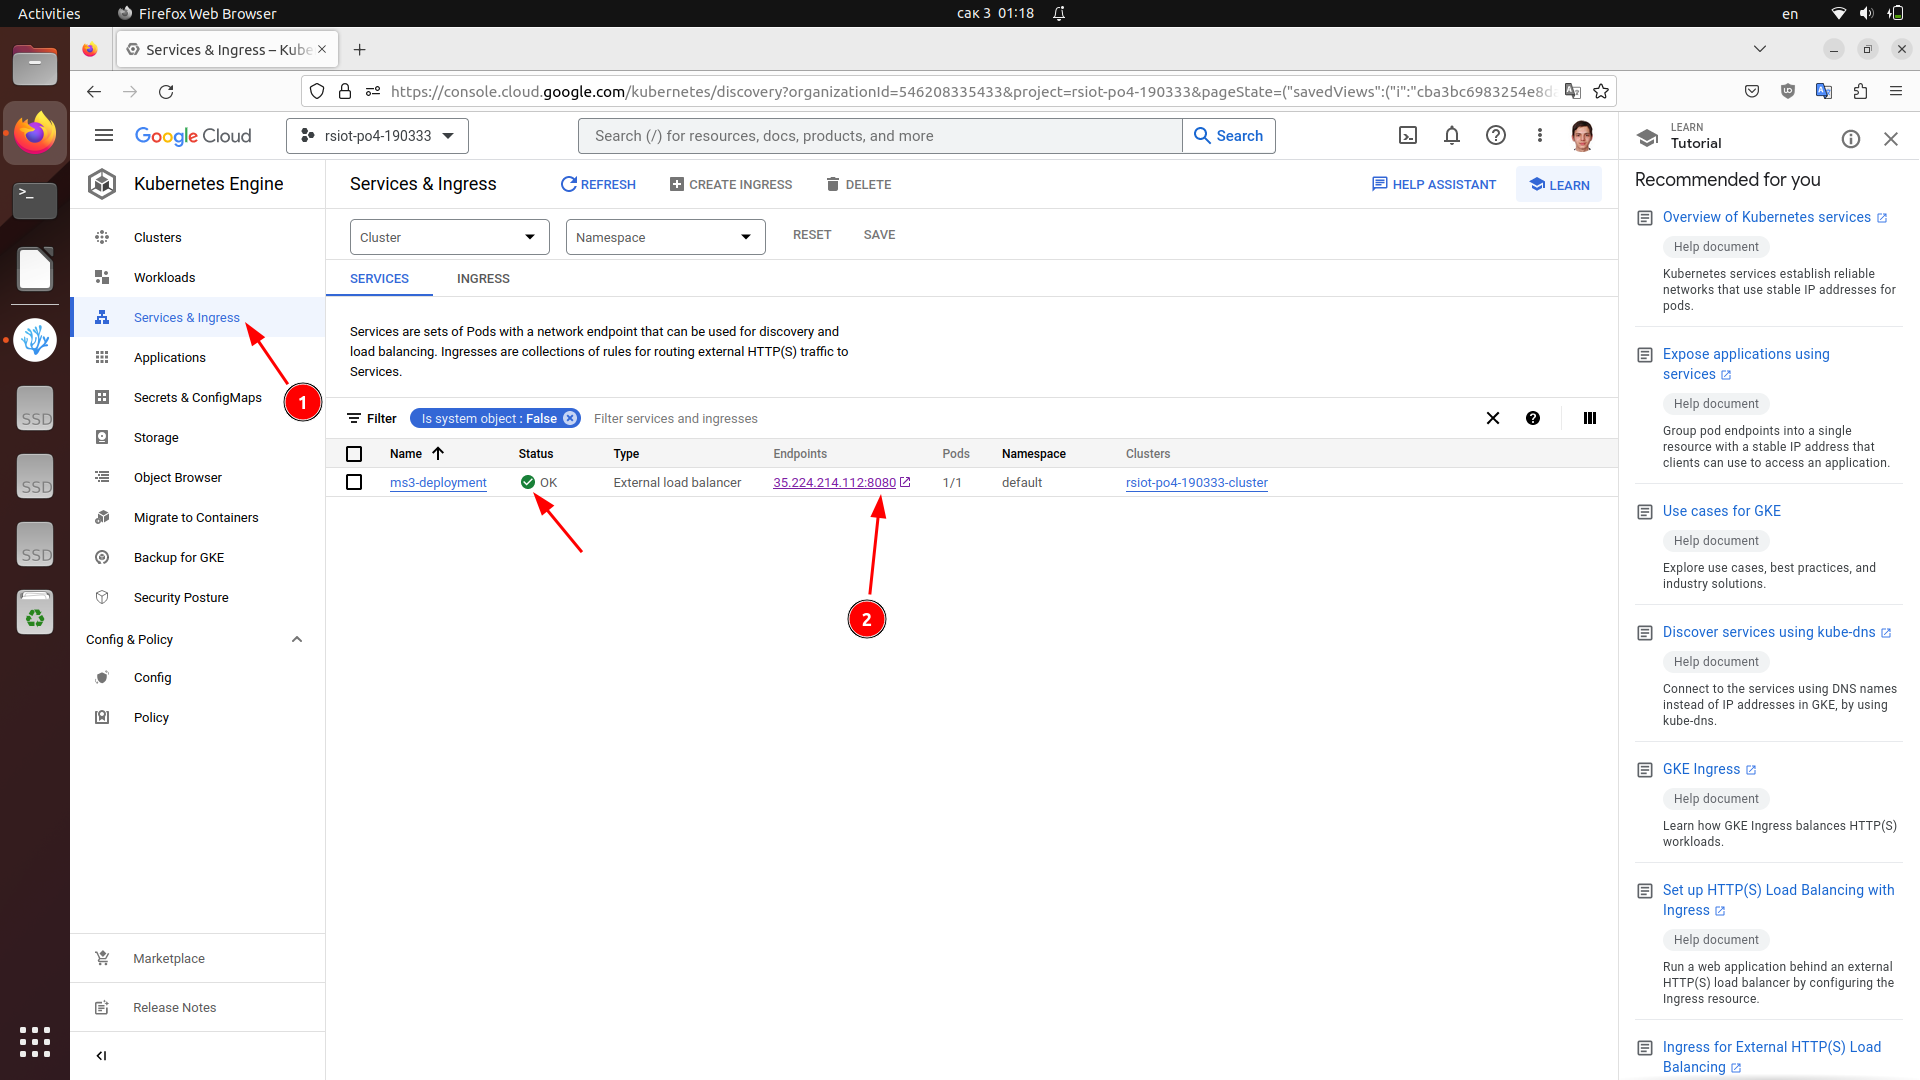
\includegraphics[height=5cm]
      {images/2023-03-03_01-19-13.png}

      \caption{\_}

      \label{fig:6}
    \end{minipage}
  \end{figure}

  Результат того, что работает MS3 на рис.~\ref{fig:7}.

  \begin{figure}[!h]
    \centering
    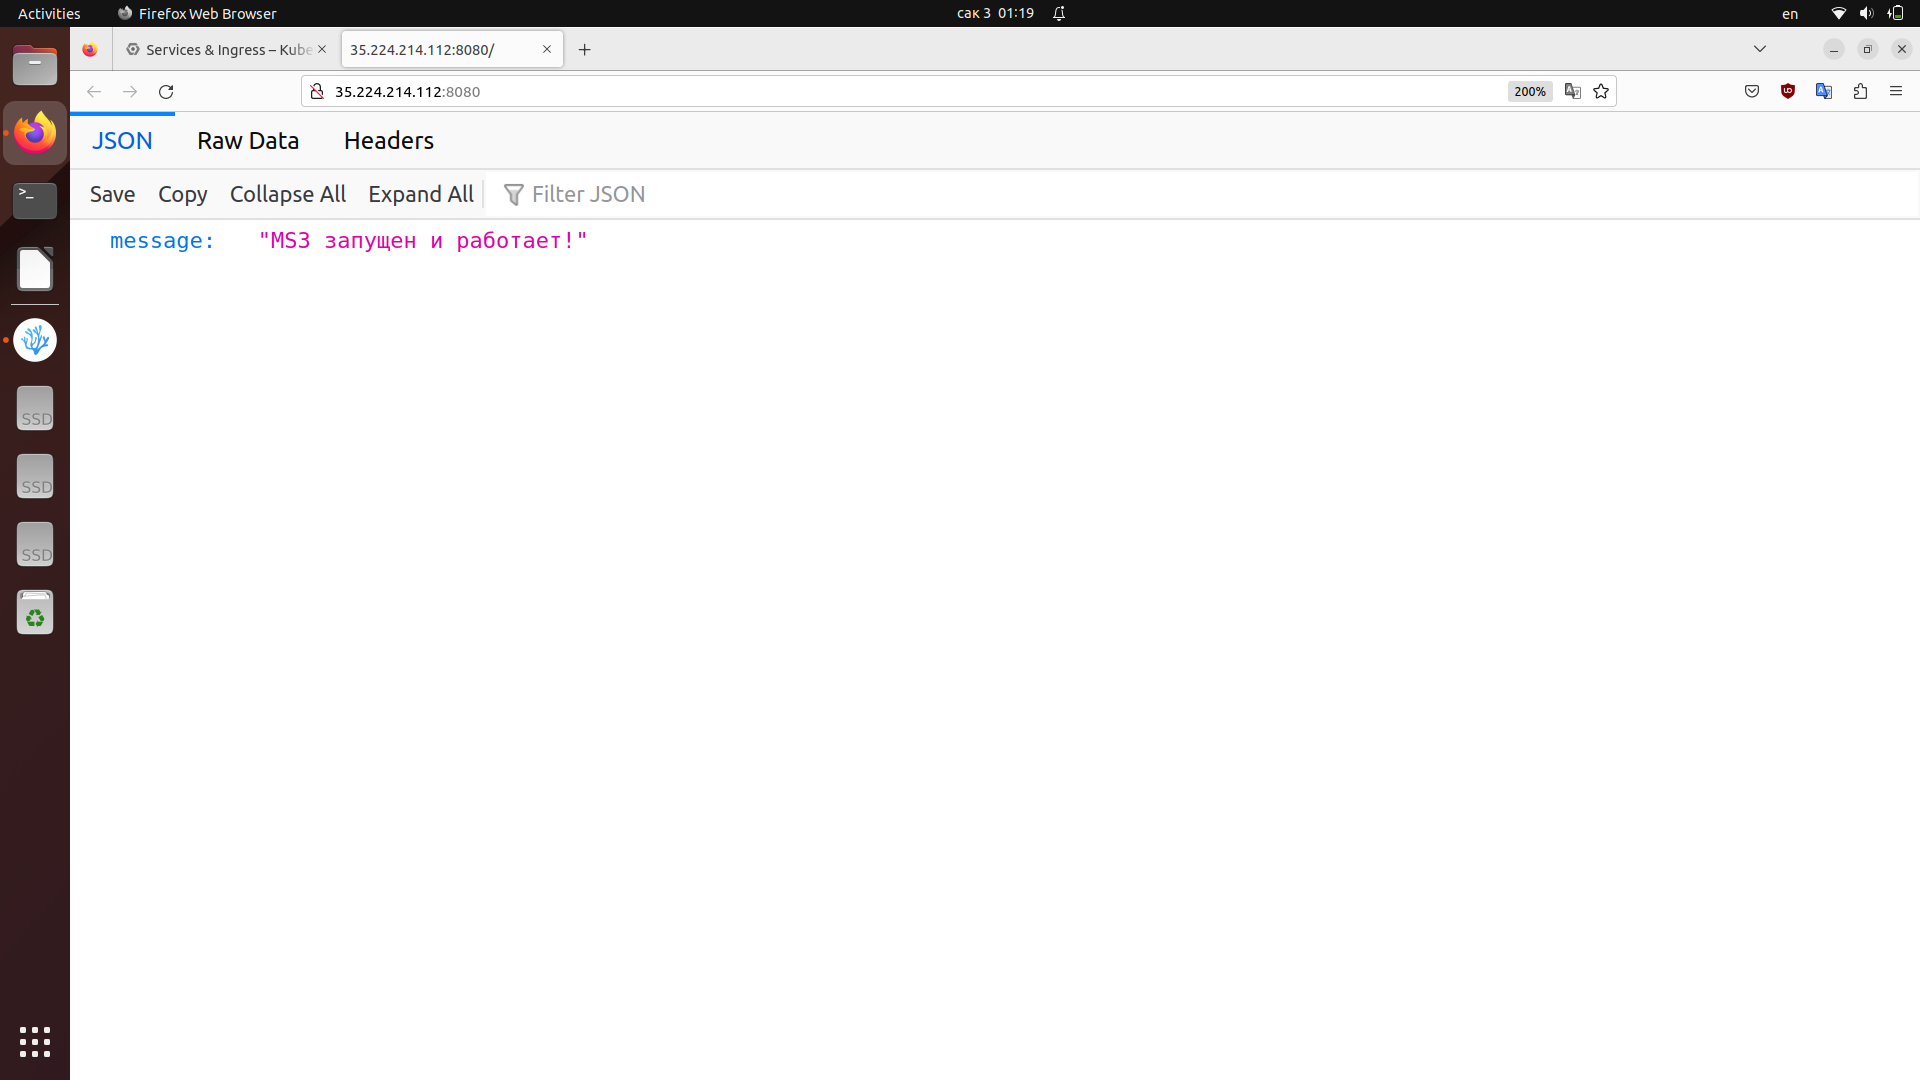
\includegraphics[width=18cm]
    {images/2023-03-03_01-19-42.png}
    \caption{\_}
    \label{fig:7}
  \end{figure}

  \newpage

  \begin{center}
    \textbf{Создание deployment в Google Cloud Kubernetes Engine для MS2}
  \end{center}

  \begin{lstlisting}[
    language=bash,
    frame=single,
    rulecolor=\color{blue},
    name={Терминал},
  ]
gcloud container clusters get-credentials rsiot-po4-190333-cluster

kubectl apply -f deployment-ms2.yaml # создаем deployment из конфига
kubectl get pods        # ждем когда будет статус Running, а не ContainerCreating
kubectl get deployments # смотрим, что создался deployment

# Можно открыть в браузере http://35.224.214.112:8080:
kubectl expose deployment ms2-deployment --type=LoadBalancer --port=80 --target-port=44480

# Можно открыть в браузере http://localhost:8888:
# $ kubectl port-forward ms2-deployment-7bbb9d8ff9-fdqzh 8888:44480

# Удалить deployment: $ kubectl delete -f deployment-ms2.yaml # удаляем deployment
\end{lstlisting}

  \lstinputlisting[
    frame=single,
    rulecolor=\color{magenta},
  ]{../sources/K8S/deployment-ms2.example.yaml}

  Как создать deployment смотрел по видео на YouTube \cite{kubernetes_create_deployment}.

  Заходим на сайт Google Cloud Kubernetes Engine \cite{GoogleCloudConsole} (см. рисунок~\ref{fig:8}).

  Жмём <<Workloads>> - и видем, что у нас запущен ms3-deployment (см. рисунок~\ref{fig:8}).

  Жмём <<Services \& Ingress>> - и видем, что у нас открыт порт (см. рисунок~\ref{fig:9}).

  \begin{figure}[!h]
    \centering

    \begin{minipage}{0.49\textwidth}
      \centering

      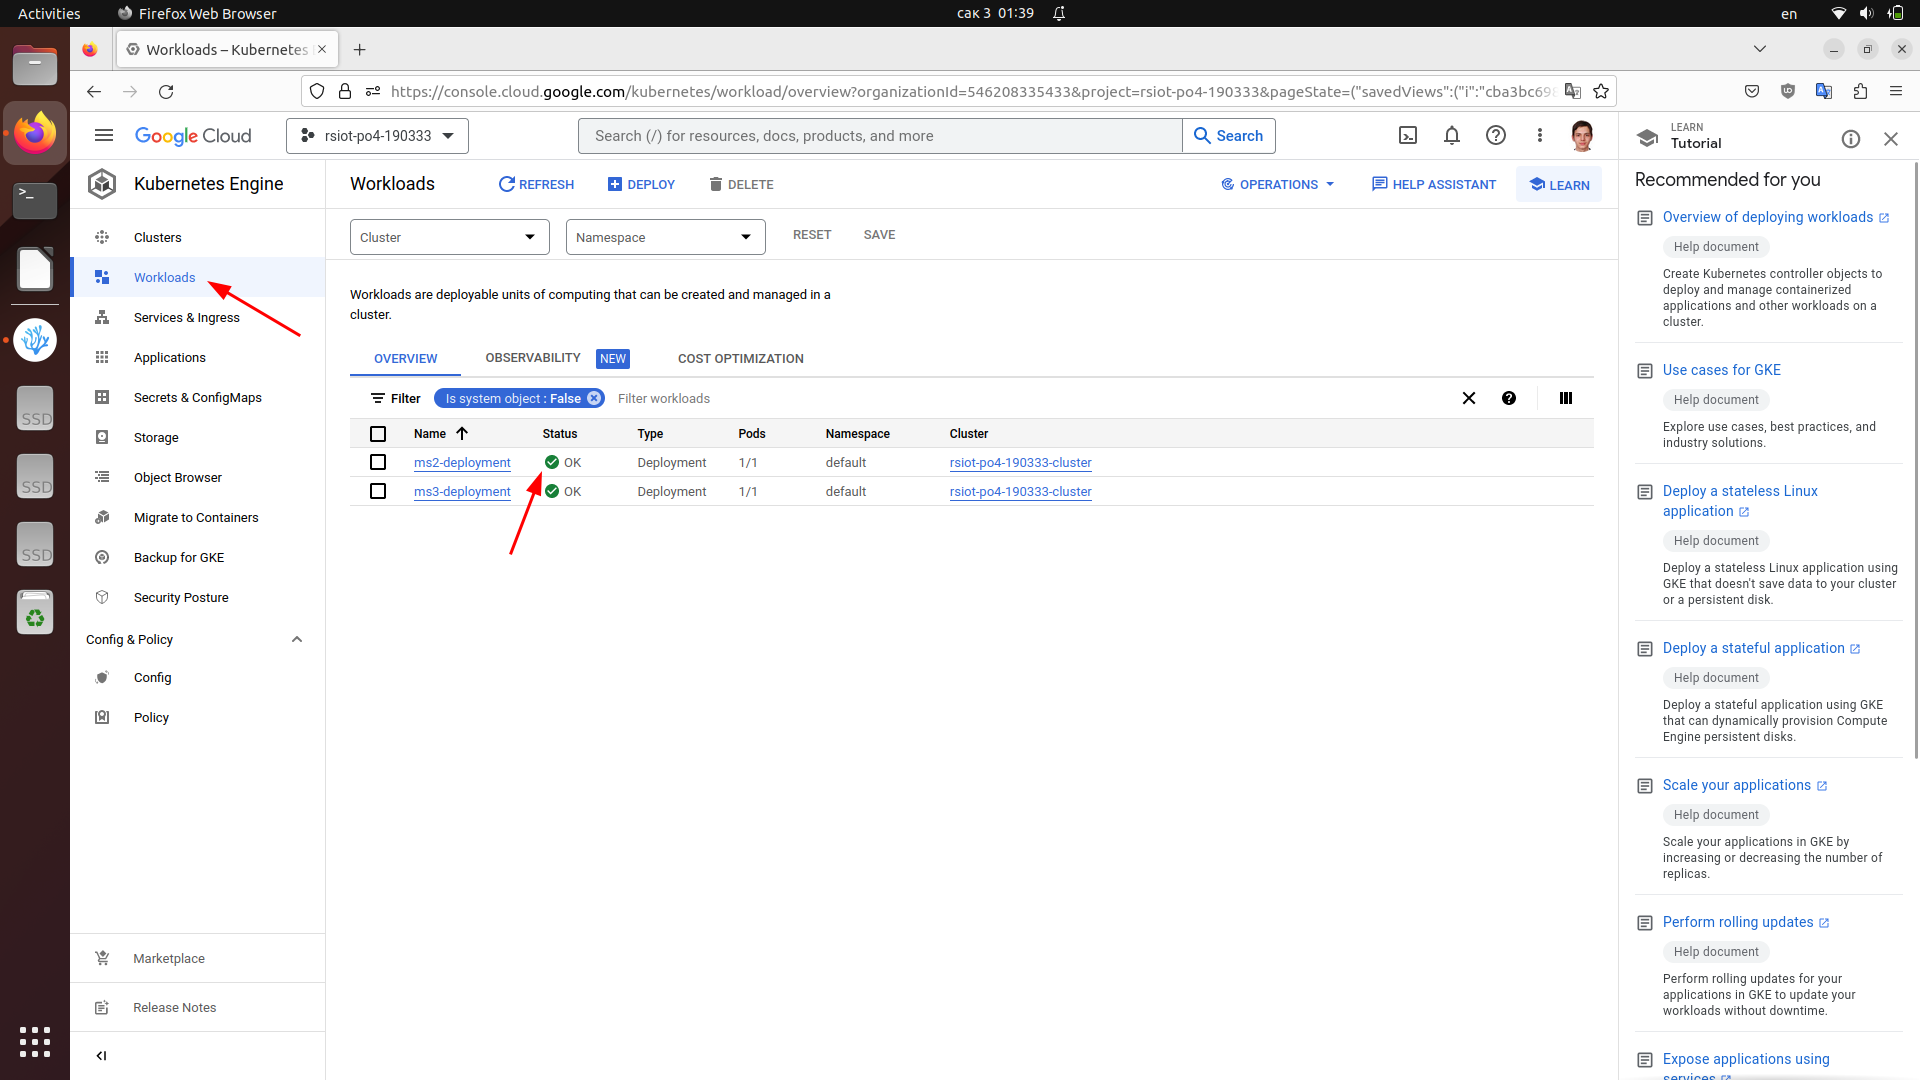
\includegraphics[height=5cm]
      {images/2023-03-03_01-40-02.png}

      \caption{\_}

      \label{fig:8}
    \end{minipage}
    \begin{minipage}{0.49\textwidth}
      \centering

      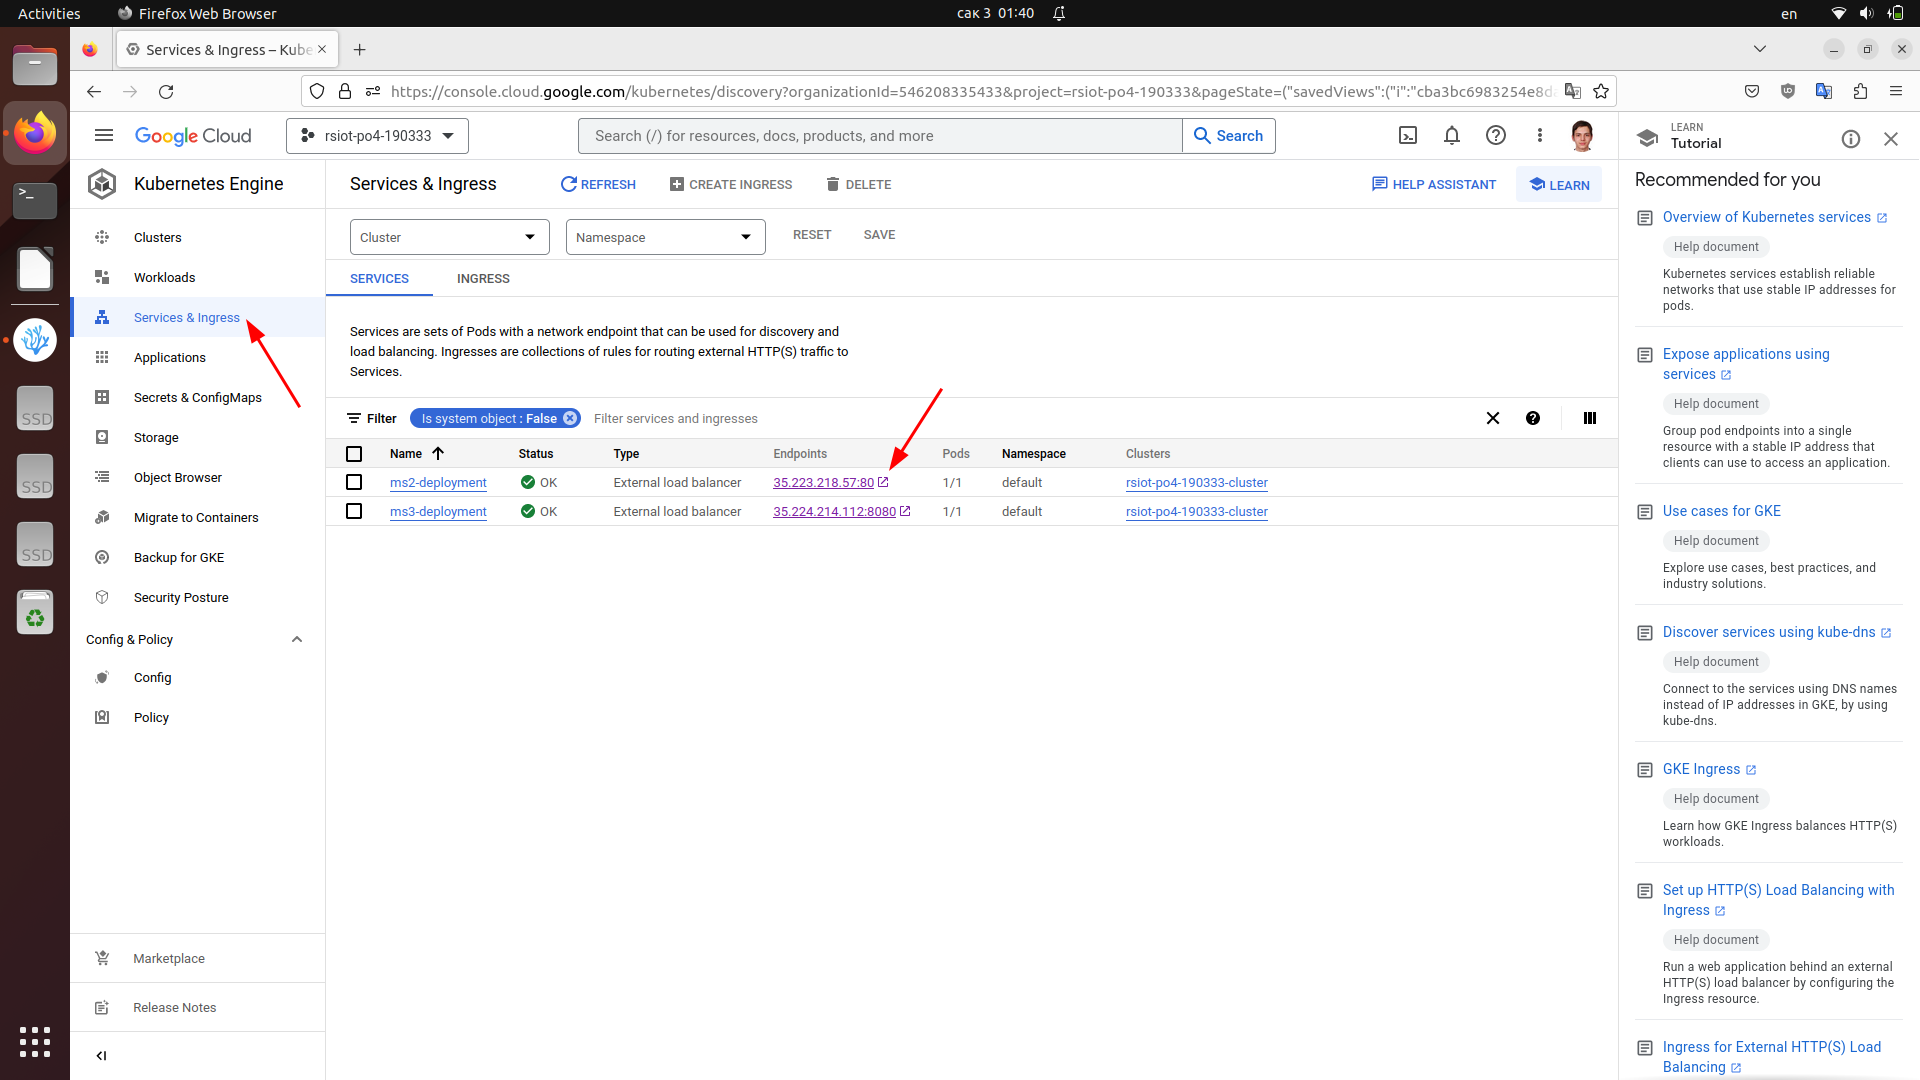
\includegraphics[height=5cm]
      {images/2023-03-03_01-40-21.png}

      \caption{\_}

      \label{fig:9}
    \end{minipage}
  \end{figure}

  Результат того, что работает MS2 на рис.~\ref{fig:10}.

  \begin{figure}[!h]
    \centering
    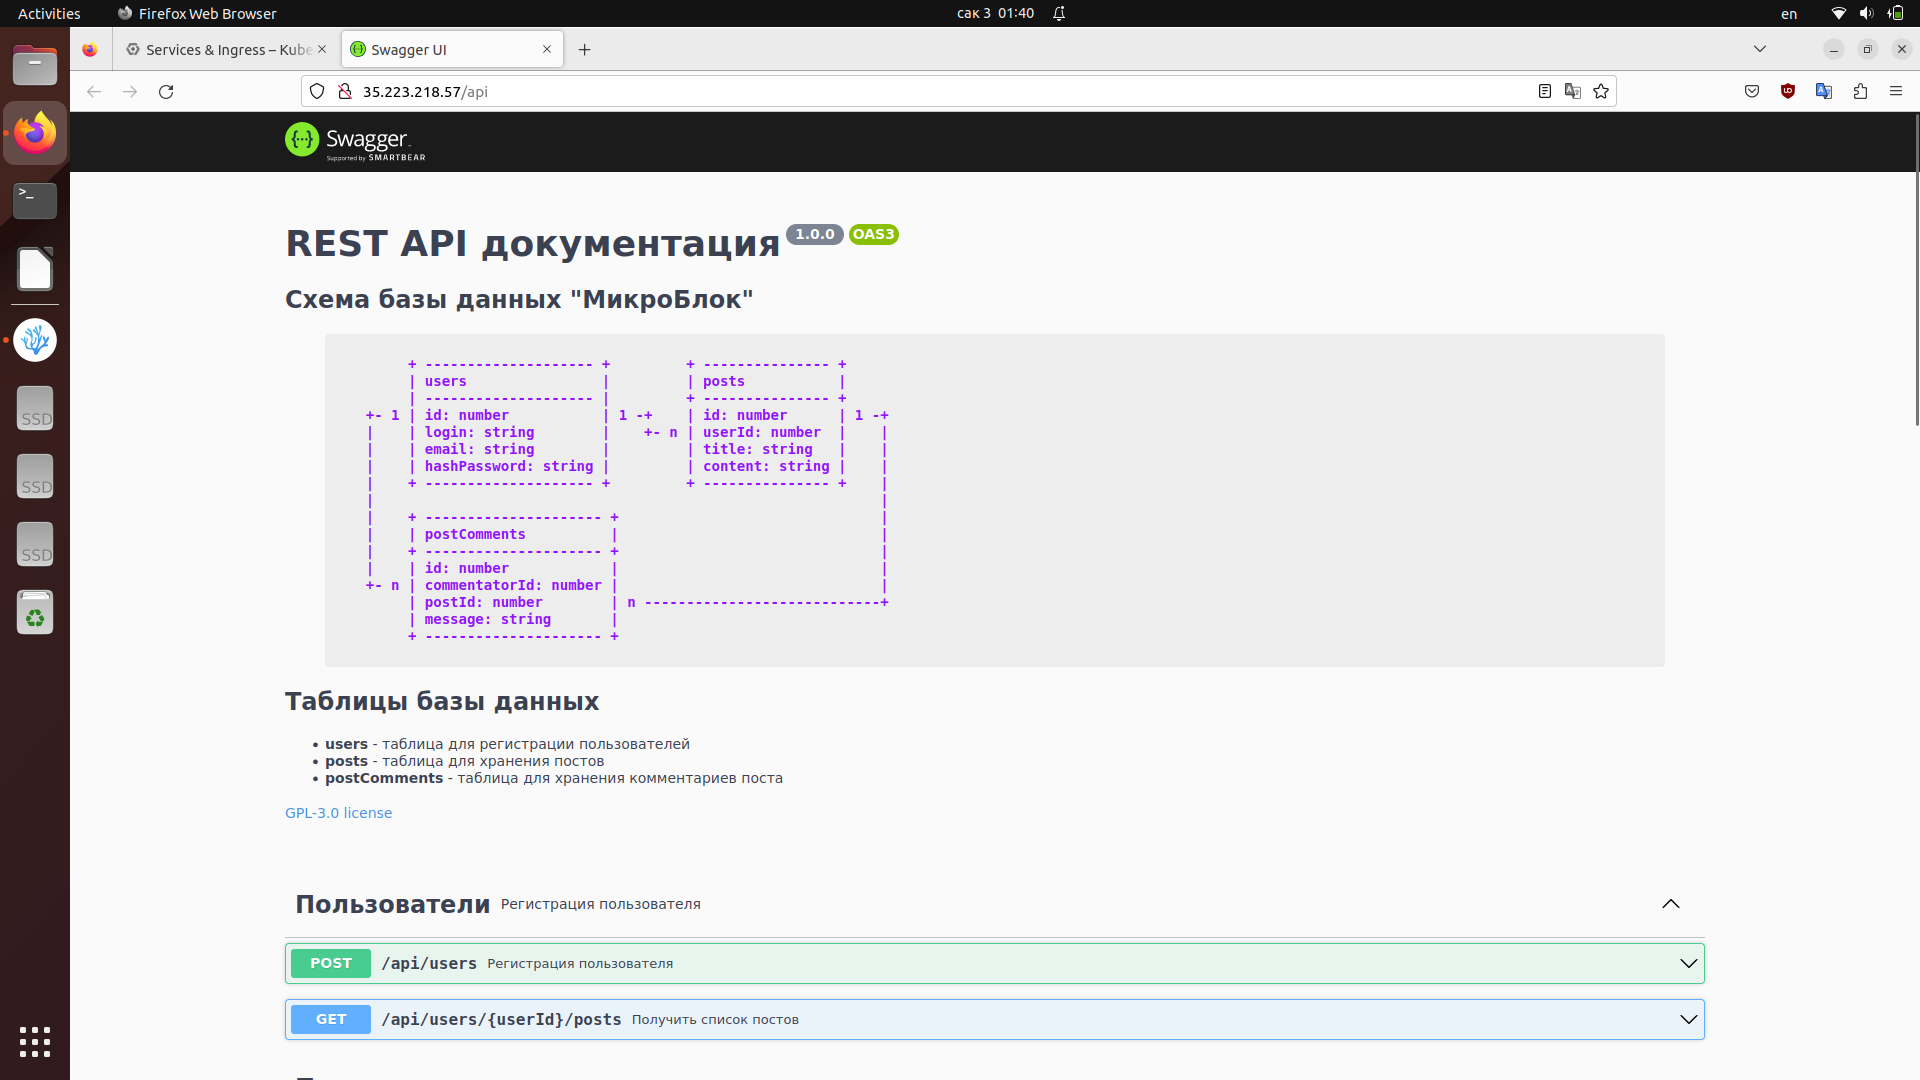
\includegraphics[width=18cm]
    {images/2023-03-03_01-40-52.png}
    \caption{\_}
    \label{fig:10}
  \end{figure}

  Для того, чтобы работала MS4 в Google Cloud Functions меняем URL на то, что открыли порт у deployment:
  http://35.223.218.57.

  \paragraph{} \textbf{Вывод}:
  Установили VirtualBox, kubectl, minikube.
  Создали кластер в VirtualBox используя minikube.
  Создали под для MS3 с помощью kubectl и конфига pod-ms3-ver1.yaml.
  Создали под для MS2 с помощью kubectl и конфига pod-ms2-ver1.yaml.
  Создали кластер в Google Cloud Kubernetes Engine.
  Сделали deployment'ы MS3 и MS2.
  Открыли порты deployment'ам.
  Проверили работу MS3 и MS2.

  % = = = = = = = = = = = = = = = =
  \newpage
  \begingroup
    \phantomsection
    \addcontentsline{toc}{section}{СПИСОК ИСПОЛЬЗОВАННЫХ ИСТОЧНИКОВ}
    \section*{Список использованных источников} %\section*{СПИСОК ИСПОЛЬЗОВАННЫХ ИСТОЧНИКОВ}

    \renewcommand{\addcontentsline}[3]{}% Remove functionality of \addcontentsline
    \renewcommand{\section}[2]{}% Remove functionality of \section

    \begin{thebibliography}{}

      \bibitem{kubernetes_install}
      2-K8s - Поднятие простого Локального K8s Cluster на Windows - YouTube
      [Электронный ресурс]. -
      Режим доступа:
      \url{https://www.youtube.com/watch?v=WAIrMmCQ3hE}.
      Дата доступа: 28.02.2023.

      \bibitem{kubernetes_install_kubectl}
      Install and Set Up kubectl on Linux | Kubernetes
      [Electronic resource]. -
      Mode of access:
      \url{https://kubernetes.io/docs/tasks/tools/install-kubectl-linux/}.
      Date of access: 28.02.2023.

      \bibitem{kubernetes_install_minikube}
      minikube start | minikube
      [Electronic resource]. -
      Mode of access:
      \url{https://minikube.sigs.k8s.io/docs/start/}.
      Date of access: 28.02.2023.

      \bibitem{kubernetes_theory}
      7-K8s - Главные Объекты Kubernetes, из чего состоит K8s - Кубернетес на простом языке - YouTube
      [Электронный ресурс]. -
      Режим доступа:
      \url{https://www.youtube.com/watch?v=ouKaU1B5eKM}.
      Дата доступа: 28.02.2023.

      \bibitem{kubernetes_create_pod}
      8-K8s - Создание и Управление - PODS - Кубернетес на простом языке - YouTube
      [Электронный ресурс]. -
      Режим доступа:
      \url{https://www.youtube.com/watch?v=kGwe8IEDiX4}.
      Дата доступа: 28.02.2023.

      \bibitem{kubernetes_create_deployment}
      9-K8s - Создание и Управление - DEPLOYMENTS - Кубернетес на простом языке - YouTube
      [Электронный ресурс]. -
      Режим доступа:
      \url{https://www.youtube.com/watch?v=l2byGad0Kk4}.
      Дата доступа: 02.03.2023.

      \bibitem{GoogleCloudConsole}
      Getting started – Google Cloud console
      [Electronic resource]. -
      Mode of access:
      \url{https://console.cloud.google.com/getting-started}.
      Date of access: 02.03.2023.

    \end{thebibliography}
  \endgroup
  % = = = = = = = = = = = = = = = =
\end{document}
